{
    \chapter{Grundlagen der Wahrscheinlichkeitstheorie}\index{Wahrscheinlichkeitstheorie|(}
    \section{Die Axiome von Kolmogorov}\index{Kolmogorov Axiome|see {Axiome von Kolmogorov}}\index{Axiome von Kolmogorov|(}

    Für das erste Beispiel im Gebiet der Wahrscheinlichkeitstheorie rollen
    wir zwei Würfel.\\

    \begin{minipage}{\linewidth}
        \centering
        \def\svgwidth{2cm}
        \input{chapters/wahrscheinlichkeitstheorie/dices.pdf_tex}\\\tiny{Steaphan Greene, CC BY-SA 3.0}
    \end{minipage}

    \begin{definition}
    Alle möglichen Ausgänge kombiniert,nennen wir \textbf{Grundmenge}.
    \end{definition}

    \textbf{Grundmenge\index{Grundmenge} $M\text{ bzw. }\Omega$}\\

    Die Grundmenge $M\text{ bzw. }\Omega$ besteht aus dem Produkt der Ausgänge von Würfel A und der Ausgänge von Würfel B:\\
    Würfel A: $A=\{1,2,3,4,5,6\}$\\
    Würfel B: $B=\{1,2,3,4,5,6\}$

    \begin{equation*}
        M=\Omega =A\times B=\{\left(1,1\right),\left(1,2\right),\ldots,\left(3,4\right),\ldots ,\left(6,6\right)\}
    \end{equation*}
    
    Egal was gewürfelt wird, unser Ergebnis ist bereits in der Grundmenge M. 
    Die Wahrscheinlichkeit \gls{symb:mathbbP} dass das Ergebnis in der Grundmenge
    liegt, ist 100\%.

    \begin{equation*}
        \mathbb{P}\left(M\right)=\mathbb{P}(\Omega )=1
    \end{equation*}

    \textbf{Elementarereignis}\index{Elementarereignis}\\
    Ein einzelner Ausgang, also z.B. $(2,5)$, wird Elementarereignis genannt.\\

    \textbf{Leere Menge \gls{symb:emptyset}}\index{Leere Menge}

    Eine leere Menge enthält kein Element. Findet jedoch ein Zug statt (z.B.
    Würfel fallen), entsteht mit Gewissheit ein Ergebnis.

    \begin{equation*}
        \mathbb{P}\left({\emptyset}\right)=0
    \end{equation*}

    Um Aussagen über bestimmte Ereignisse treffen zu können, können wir nun
    {\quotedblbase}Ergebnismengen{\textquotedblleft} konstruieren, die nur
    für uns interessante Elementarereignisse enthalten. Beispielsweise
    interessieren uns alle Würfe, bei denen die Summe der Augenzahlen 9
    ergibt. Nun nehmen wir uns genau diese Elementarereignisse aus der
    Grundmenge: (siehe Abbildung \ref{fig:teilmenge1})

    \begin{equation*}
        A=\{\left(3,6\right),\left(4,5\right),\left(5,4\right),\left(6,3\right)\}
    \end{equation*}

    \begin{figure}
    \subfigure[Teilmenge $A\subset \Omega$]{
        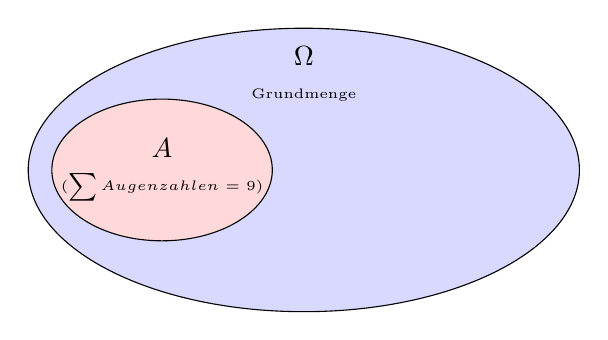
\begin{tikzpicture}
            {
    \def\ninecircle{(-1.8,0) ellipse (1.4cm and 0.9cm)}
    \def\omegacircle{(0,0) ellipse (3.5cm and 1.8cm)}

    \fill[blue!15] \omegacircle;
    \fill[red!15] \ninecircle;

    \draw \omegacircle node[above=0.75cm, text width=2.8cm,align=center] {$\Omega$\\\tiny{Grundmenge}};
    \draw \ninecircle node[text width=2.8cm,align=center] {$A$\\\tiny{($\sum\text{Augenzahlen}=9$)}};
}

        \end{tikzpicture}
        \label{fig:teilmenge1}
    }
    \subfigure[Teilmenge $A\subset \Omega$ und Teilmenge $B\subset \Omega$]{
        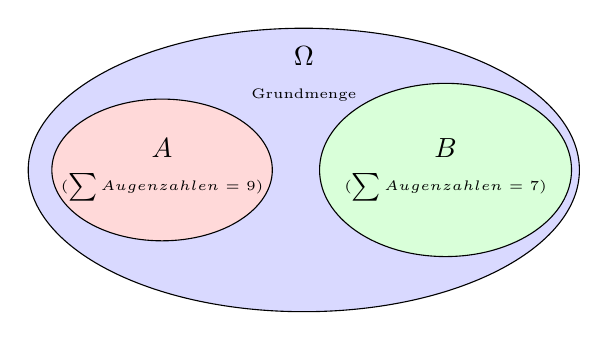
\begin{tikzpicture}
            {
    \def\ninecircle{(-1.8,0) ellipse (1.4cm and 0.9cm)}
    \def\sevencircle{(+1.8,0) ellipse (1.6cm and 1.1cm)}
    \def\omegacircle{(0,0) ellipse (3.5cm and 1.8cm)}

    \fill[blue!15] \omegacircle;
    \fill[red!15] \ninecircle;
    \fill[green!15] \sevencircle;

    \draw \omegacircle node[above=0.75cm, text width=2.8cm,align=center] {$\Omega$\\\tiny{Grundmenge}};
    \draw \ninecircle node[text width=2.8cm,align=center] {$A$\\\tiny{($\sum\text{Augenzahlen}=9$)}};
    \draw \sevencircle node[text width=2.8cm,align=center] {$B$\\\tiny{($\sum\text{Augenzahlen}=7$)}};
}

        \end{tikzpicture}
        \label{fig:teilmenge2}
    }
    \label{fig:teilmengen}
    \caption{Teilmengen der Grundmenge $\Omega$}
    \end{figure}

    Wir arbeiten also mit Mengen, die eine bestimmte Wahrscheinlichkeit
    besitzen. Im besten Fall enthält die Menge alle Elemente, im
    schlechtesten Fall keine. Es gilt:
    \begin{equation*}
        0\le \mathbb{P}\left(A\right)\le 1
    \end{equation*}
    Zusätzlich geben wir uns auch zufrieden, wenn die Summe der Augenzahlen 7 ergibt. (siehe Abbildung \ref{fig:teilmenge2})

    \begin{equation*}
        B=\{\left(1,6\right),\left(2,5\right),\left(3,4\right),\left(4,3\right),\left(5,2\right),\left(6,1\right)\}
    \end{equation*}

    Diese Mengen sind \textbf{disjunkt}\index{disjunkte Mengen}, besitzen also keine gleichen Elemente. Die
    Wahrscheinlichkeit, dass $A$ oder $B$ eintrifft, kann durch die einfache
    Addition der einzelnen Wahrscheinlichkeiten berechnet werden:

    \begin{equation*}
        \mathbb{P}(A\cup B)=\mathbb{P}\left(A\right)+\mathbb{P}\left(B\right)
    \end{equation*}
    \begin{equation*}
        0\le \mathbb{P}\left(A\right)\le \mathbb{P}\left(B\right)\le \mathbb{P}\left(A+B\right)\le 1
    \end{equation*}
    \begin{definition}[$\sigma$-Algebra]\index{sigma-Algebra@$\sigma$-Algebra}:

        Da wir später öfters noch den Begriff  $\sigma$-Algebra brauchen werden, möchte ich
        sie zuerst allgemein definieren. Diese Algebra kommt aus der
        Mengenlehre und besitzt drei wichtige Eigenschaften:

        \begin{itemize}
            \item $\Omega \in \mathcal S$
            \item Ist $A\in \mathcal S$ dann ist auch $A^{C}\in \mathcal S$
            \item Sind $A_{i}\in \mathcal S,\,i\in \mathbb{N}$, so ist auch $\cup _{i=1}^{{\infty}}A_{i}\in \mathcal S$
        \end{itemize}
    \end{definition}
    Angenommen wir werfen eine Münze. Dann ist die Grundmenge $\Omega$ 
    (manchmal auch \textbf{Obermenge}\index{Obermenge} bezeichnet):
    \begin{equation*}
        \Omega =\{K,Z\}
    \end{equation*}

    und die Elementarereignisse $\{K\}$ und $\{Z\}$ Nur was ist jetzt $\mathcal S$? Ohne
    weitere Angaben gilt:

    \begin{equation*}
        \mathcal S=\{\emptyset,\{K\},\{Z\},\{K,Z\}\}
    \end{equation*}


    \begin{bsp}\label{bsp:wuerfel}
        Angenommen wir werfen einen Würfel:
        \begin{equation*}
            \Omega=\{1,2,3,4,5,6\}
        \end{equation*}
        und die Elementarereignisse $\{1\},\{2\},...,\{6\},$. Ohne weitere Einschränkungen gilt
        \[\mathcal S=\{\emptyset,\{1\},...,\{1,2\},...,\{2,4,5\},...,\{1,2,5,6\},...,\{1,2,3,4,6\},...,\{1,2,3,4,5,6\}\}\]

        $\mathcal S$ muss jedoch nicht immer die gesamte Potenzmenge sein. Möchten wir nur folgenden Fälle betrachten:
        \begin{eqnarray*}
            A &=& \{2,4,6\}=\text{Gerade Zahl wird geworfen}\\
            B &=& \{1,3,5\}=\text{Ungerade Zahl wird geworfen}\\
        C &=& \{6\}
        \end{eqnarray*}
        Diese Algebra besteht aus $2^3$ Elementen:
        \begin{equation*}
            \mathcal S=\{\emptyset,\{6\},\{2,4,6\},\{1,3,5\},\{1,3,5,6\},\{1,2,3,4,5\},\{1,2,3,4,5,6\}\}
        \end{equation*}
        Die einzelnen Elemente lassen sich direkt aus den Eigenschaften einer $\sigma$-Algebra erstellen.
    \end{bsp}
    
    Mit diesem Wissen können wir uns nun den Axiomen von Kolmogorov zuwenden.

    \begin{definition}[Axiome von Kolmogorov]\label{def:axiome_kolmogorov}:
        \index{Axiome von Kolmogorov}
        Ist  $\Omega$ eine Grundmenge und $\mathcal S$ eine $\sigma$-Algebra von $\Omega$. Eine Abbildung
        \begin{equation*}
            \mathbb{P}:\mathcal S\rightarrow \mathbb{R}
        \end{equation*}
        heißt \textbf{Wahrscheinlichkeit}\index{Wahrscheinlichkeit} oder \textbf{Wahrscheinlichkeitsmaß}\index{Wahrscheinlichkeitsmaß}, wenn $\mathbb{P}$ die folgenden drei Eigenschaften besitzt:

        \begin{enumerate}
            \item Wahrscheinlichkeit einer beliebigen Menge zwischen 0 und 1:\\
                $\forall A\in \mathcal S: 0\leq\mathbb{P}(A)\leq 1$
            \item Wahrscheinlichkeit der leeren Menge ist 0:\\
                $\mathbb P\left({\emptyset}\right)=0$
            \item Ergebnis ist immer in der Grundmenge:\\ 
                $\mathbb P\left(\Omega \right)=1$
            \item Addition von disjunkten Mengen:\\
                Wenn $A_{n},n\in\mathbb{N}$ disjunkte Mengen sind, dann gilt:
                \[\mathbb{P}\left(\bigcup_{n\in\mathbb{N}}A_n\right)=\sum_{n\in\mathbb{N}}\mathbb{P}(A_n)\]
        \end{enumerate}
        Das Tripel $(\Omega, \mathcal S, \mathbb{P})$ heißt \textbf{Wahrscheinlichkeitsraum}\index{Wahrscheinlichkeitsraum}.
    \end{definition}

    Bei unserem Würfelspiel (siehe Beispiel \ref{bsp:wuerfel}) mit den zwei geworfenen Würfeln können wir noch
    weitere Eigenschaften feststellen. Einerseits gibt es endlich viele
    mögliche Ausgänge ($|\Omega|<{\infty}$), andererseits
    besitzt jede Kombination $k$ die gleiche Wahrscheinlichkeit (${|\Omega|=36\Rightarrow}$\\
    ${\mathbb{P}\left(k\right)=\frac{1}{|\Omega|}=\frac{1}{36}}$) und
    schlussendlich schließen sich die Ereignisse aus. In Tabelle \ref{tab:wuerfeln} sieht man alle möglichen Kombinationen sowie jede Einzelwahrscheinlichkeit.

\begin{table}
    \centering
    \begin{tabular}{|c|c|c|c|c|c|c|}
        \hline
        \diagbox{Würfel 1}{Würfel 2} & 1 & 2 & 3 & 4 & 5 & 6\\
        \hline
        1 & $\frac{1}{16}$ & $\frac{1}{16}$ & $\frac{1}{16}$ & $\frac{1}{16}$ & $\frac{1}{16}$ & $\frac{1}{16}$\\
        \hline
        2 & $\frac{1}{16}$ & $\frac{1}{16}$ & $\frac{1}{16}$ & $\frac{1}{16}$ & $\frac{1}{16}$ & $\frac{1}{16}$\\
        \hline
        3 & $\frac{1}{16}$ & $\frac{1}{16}$ & $\frac{1}{16}$ & $\frac{1}{16}$ & $\frac{1}{16}$ & $\frac{1}{16}$\\
        \hline
        4 & $\frac{1}{16}$ & $\frac{1}{16}$ & $\frac{1}{16}$ & $\frac{1}{16}$ & $\frac{1}{16}$ & $\frac{1}{16}$\\
        \hline
        5 & $\frac{1}{16}$ & $\frac{1}{16}$ & $\frac{1}{16}$ & $\frac{1}{16}$ & $\frac{1}{16}$ & $\frac{1}{16}$\\
        \hline
        6 & $\frac{1}{16}$ & $\frac{1}{16}$ & $\frac{1}{16}$ & $\frac{1}{16}$ & $\frac{1}{16}$ & $\frac{1}{16}$\\
        \hline
    \end{tabular}
    \caption{Würfelergenisse und Wahrscheinlichkeiten mit 2 Würfeln (Beispiel \ref{bsp:wuerfel})}\label{tab:wuerfeln}
\end{table}

    Das führt uns zur Definition eines Laplace-Experiments:
    \begin{definition}[Laplace-Experiment]\index{Laplacescher Wahrscheinlichkeitsraum}\index{Laplace-Experiment|see{Laplacescher Wahrscheinlichkeitsraum}}:\\
        Im Laplace-Experiment mit endlich vielen Ausgängen besitzt jeder Ausgang
        die gleiche Wahrscheinlichkeit.
        \begin{equation*}
            \mathbb{P}(A)=\frac{|A|}{|M|}
        \end{equation*}
    \end{definition}

    \begin{definition}[Weitere Eigenschaften aus den Axiomen von Kolmogorov]:\\
        \index{Axiome von Kolmogorov!weitere Eigenschaften}
        \begin{enumerate}
            \item Wahrscheinlichkeit, dass $A$ nicht auftritt:\\
                $\mathbb{P}\left(A^{C}\right)=1-\mathbb{P}(A)$
            \item $A$ ist eine Teilmenge von $B$ ($A\subseteq B)$\\
                Wenn $A\subseteq B$, dann gilt: $\mathbb{P}(A)\le \mathbb{P}(B)$
            \item Vereinigung von $A$ und $B$:\\
                $\mathbb{P}(A\cup B)=\mathbb{P}(A)+\mathbb{P}(B)-\mathbb{P}(A\cap B)$
            \item Vereinigung ist kleiner, gleich der Summe
                \[\text{Für }A_n\subseteq A_{n+1}:\;\;\mathbb{P}\left(\bigcup_nA_n\right)=\lim_n\mathbb{P}(A_n)\]
                \[\text{Für }A_n\subseteq A_{n+1}:\;\;\mathbb{P}\left(\bigcup_nA_n\right)\leq\sum_n\mathbb{P}(A_n)\]
        \end{enumerate}
    \end{definition}

    \textbf{Additionstheorem}\\
    Als Anwendung des Satzes \ref{satz:additionstheorem} berechnen wir die Wahrscheinlichkeit, dass
    eine zufällig gewählte Permutation von $n$ Elementen keinen Fixpunkt hat.
    Das Additionstheorem scheint auf den ersten Blick etwas kompliziert zu
    sein, ist aber ein einfaches Schema, das nur wiederholt werden muss.

    \begin{satz} \textbf{Additionstheorem}\index{Additionstheorem}\index{Siebformel}
    \label{satz:additionstheorem}
    \[\mathbb{P}\left(\bigcup_{i=1}^nA_i\right)=\sum_{i=1}^n(-1)^{i-1}S_i\]
    \[\text{mit } S_i=\sum_{i\leq j_1\leq j_2\leq ...\leq j_i\leq n} \mathbb{P}(A_{j_1}\cap...\cap A_{j_i})\]
    Also somit:
    \[\mathbb{P}(\bigcup_i A_i)=\sum_i\mathbb{P}(A_i)-\sum_{i<j}\mathbb{P}(A_i\cap A_j)+\sum_{i<j<k}\mathbb{P}(A_i\cap A_j\cap A_k)-+...\]
    \end{satz}

    Vorher haben wir gesagt, dass zwei disjunkte Mengen
    einfach addiert werden können. Sind diese jedoch nicht vollständig
    disjunkt, es existieren also Elemente, die in beiden Mengen enthalten
    sind, so würden manche Elemente mehrmals gezählt werden. Das Beispiel \ref{bsp:ehepaare_tanzen} 
    verdeutlicht dieses Problem genauer.

    \textbf{Formale Berechnung: Wahrscheinlichkeit, dass kein Fixpunkt existiert}

    Im Beispiel \ref{bsp:ehepaare_tanzen} ist ein Fixpunkt ein Ehepaar, das nach dem
    Signal zusammen bleibt. Wir benutzen in solchen Beispielen die
    Gegenwahrscheinlichkeit, betrachten den Fall, dass mindestens ein
    Fixpunkt $A$ existiert.

    Vereinigung aller Wahrscheinlichkeiten, dass ein Fixpunkt existiert: 

    \begin{equation*}
        \mathbb{P}\left(A\right)=\mathbb{P}\left(\overset{n}{\underset{i=1}{{\bigcup}}}A_{i}\right)=\sum
    _{i=1}^{n}\left(-1\right)^{i-1}S_{i}
    \end{equation*}

    Dafür müssen wir die Summanden $S_{k}$ berechnen. Das Ereignis $A_{1}\cap ... \cap A_{k}$ tritt ein, wenn
    $j_1,...,j_n$ Fixpunkte sind, die anderen $n-k$ Elemente können beliebig vertauscht werden. Es gibt $(n-k)!$
    Möglichkeiten, diese anzuordnen. Insgesamt existieren $n!$ Möglichkeiten, die Wahrscheinlichkeit ist also
    $\frac{(n-k)!}{n!}$. Außerdem existieren $\binom{n}{k}$ Möglichkeiten, aus $n$ Paaren, $k$ auszuwählen. 
    Wir schreiben für $S_{k}$:

    \[S_{k}=\binom{n}{k}\frac{(n-k)!}{n!}=\frac{1}{k!}\]

    Somit können wir $\mathbb P\left(A\right)$ und die eigentlich wichtigere Wahrscheinlichkeit 
    $\mathbb P\left(A^C\right)$ berechnen:

    \[
    \mathbb P\left(A\right)=\sum_{k=1}^{n}\left(-1\right)^{k-1}\frac{1}{k!}\Rightarrow
    \mathbb P\left(A^{C}\right)=1-\mathbb{P}\left(A\right)=\sum_{k=0}^{n}{\left(-1\right)^{k}\frac{1}{k!}}
    \]
    Die Umformung kann überprüft werden,
    indem die ersten paar Summanden aufgeschrieben werden. Für große $n$ konvergiert die Reihe gegen
    $\frac{1}{e}$.
    Die Näherung ist so gut, dass sich die Anzahl der Permutationen ohne
    Fixpunkt (für $n\ge1$) bestimmen lässt, indem man $\frac{n!}{e}$
    auf die nächste ganze Zahl rundet.
    \newpage
    \begin{bsp}[Ehepaare tanzen (Additionstheorem)]\label{bsp:ehepaare_tanzen}

    Nun stellen wir uns folgende Situation vor: Drei Ehepaare tanzen
    zusammen. Nach einer Weile ertönt ein Signal, die Namen aller Männer
    werden in ein Topf geworfen und jede Frau darf sich einen Namen ziehen.
    Nun stellt sich uns die Frage, wie hoch die Wahrscheinlichkeit ist,
    dass kein Ehepaar miteinander tanzt.

    Dafür benutzen wir die Gegenwahrscheinlichkeit, $\mathbb P\left(\text{kein Ehepaar tanzt}\right)$ ergibt sich durch 
    $1-\mathbb P\left(\text{mind. ein Ehepaar tanzt}\right)$.

    \textbf{Ich definiere:}
    \[\mathbb P\left(E_{i}\right)=\text{Ehepaar $i$ tanzt nach dem Signal weiterhin miteinander}\]

    Der schwarze Rahmen in Abbildung \ref{fig:tanzen1} steht für alle
    Ausgangsmöglichkeiten nach dem Signal, er ist die Grundmenge $\Omega$. Darin
    befinden sich drei Kreise, jeder Kreis beinhaltet die
    Wahrscheinlichkeit, dass das entsprechende Ehepaar weiterhin
    miteinander tanzt.

    Wie bereits erwähnt, benutzen wir die Gegenwahrscheinlichkeit. Dafür
    müssen wir die orange Fläche in Abbildung \ref{fig:tanzen2} berechnen.

    Instinktiv würden wir jetzt folgende Gleichung aufschreiben:

    \[
        1-\mathbb{P}\left(\text{min. ein Ehepaar tanzt}\right)=1-\mathbb{P}(E_1)+\mathbb{P}(E_2)+\mathbb{P}(E_3)
    \]
    Jedoch wurden einige Flächenelemente doppelt gezählt. Diese sind in Abbildung \ref{fig:tanzen3} orange gekennzeichnet:

    Damit unsere Gleichung wieder stimmt, müssen wir diese abziehen:

    \begin{eqnarray*}
         &1-\mathbb{P}\left(\text{min. ein Ehepaar tanzt}\right)=\\
         &=1-\mathbb{P}(E_1)+\mathbb{P}(E_2)+\mathbb{P}(E_3)-\mathbb{P}(E_1\cap E_2)-\mathbb{P}(E_1\cap E_3)-\mathbb{P}(E_2\cap E_3)
    \end{eqnarray*}
    Nun fehlt uns nur noch eine kleine Korrektur, denn durch den letzten
    Schritt haben wir das kleine Mittelstück einmal zu viel abgezogen.

    \begin{eqnarray*}
         &1-\mathbb{P}\left(\text{min. ein Ehepaar tanzt}\right)=\\
         &=1-\mathbb{P}(E_1)+\mathbb{P}(E_2)+\mathbb{P}(E_3)-\mathbb{P}(E_1\cap E_2)-\mathbb{P}(E_1\cap E_3)\\
         &-\mathbb{P}(E_2\cap E_3)+\mathbb{P}(E_1\cap E_2\cap E_3)
    \end{eqnarray*}
	\end{bsp}

    \begin{figure}
    \centering
    \subfigure[Ehepaare $E_1-E_3$ als Teilmengen von $\Omega$]{
        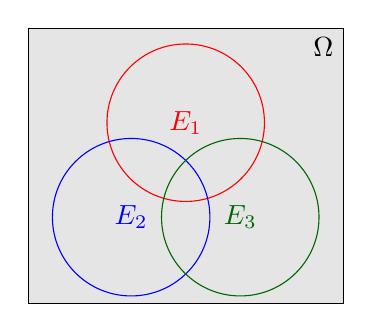
\begin{tikzpicture}
            {
    \def\firstcircle{(90:0.8cm) circle (1cm)}
    \def\secondcircle{(210:0.8cm) circle (1cm)}
    \def\thirdcircle{(330:0.8cm) circle (1cm)}
    \def\rectangle{(-2,-1.5) rectangle (2,2)}

    \fill[black!10] \rectangle;

    \draw[red] \firstcircle node {$E_1$};
    \draw[blue] \secondcircle node {$E_2$};
    \draw[green!40!black] \thirdcircle node {$E_3$};
    \draw[black] \rectangle node[below left,black] {$\Omega$};
}

        \end{tikzpicture}
        \label{fig:tanzen1}
    }
    \subfigure[Fläche, die für Gegenwahrscheinlichkeit berechnet werden soll]{
        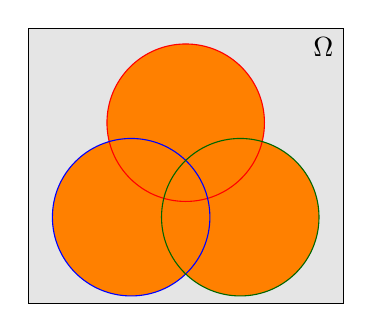
\begin{tikzpicture}
            {
    \def\firstcircle{(90:0.8cm) circle (1cm)}
    \def\secondcircle{(210:0.8cm) circle (1cm)}
    \def\thirdcircle{(330:0.8cm) circle (1cm)}
    \def\rectangle{(-2,-1.5) rectangle (2,2)}

    \fill[black!10] \rectangle;
    \fill[orange] \firstcircle;
    \fill[orange] \secondcircle;
    \fill[orange] \thirdcircle;

    \draw[red] \firstcircle;
    \draw[blue] \secondcircle;
    \draw[green!40!black] \thirdcircle;
    \draw[black] \rectangle node[below left,black] {$\Omega$};
}

        \end{tikzpicture}
        \label{fig:tanzen2}
    }
    \subfigure[Fläche, die doppelt gezählt wurde]{
        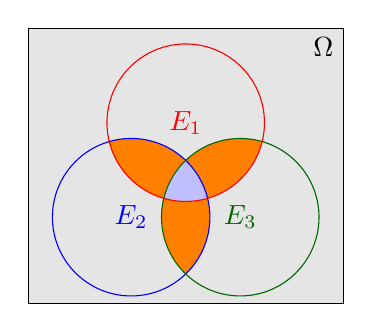
\begin{tikzpicture}
            {
    \def\firstcircle{(90:0.8cm) circle (1cm)}
    \def\secondcircle{(210:0.8cm) circle (1cm)}
    \def\thirdcircle{(330:0.8cm) circle (1cm)}
    \def\rectangle{(-2,-1.5) rectangle (2,2)}

    \fill[black!10] \rectangle;
    \fill[black!10] \firstcircle;
    \fill[black!10] \secondcircle;
    \fill[black!10] \thirdcircle;

    \begin{scope}
        \clip \firstcircle;
        \fill[orange] \secondcircle;
    \end{scope}
    \begin{scope}
        \clip \firstcircle;
        \fill[orange] \thirdcircle;
    \end{scope}
    \begin{scope}
        \clip \secondcircle;
        \fill[orange] \thirdcircle;
    \end{scope}

    \begin{scope}
        \clip \firstcircle;
        \clip \secondcircle;
        \fill[blue!25] \thirdcircle;
    \end{scope}

    \draw[red] \firstcircle node {$E_1$};
    \draw[blue] \secondcircle node {$E_2$};
    \draw[green!40!black] \thirdcircle node {$E_3$};
    \draw[black] \rectangle node[below left,black] {$\Omega$};
}

        \end{tikzpicture}
        \label{fig:tanzen3}
    }
    \label{fig:teilmengen}
    \caption{Der Kreis $E_1$ gibt z.B. die Wahrscheinlichkeit an, dass das Ehepaar $E_1$ nach dem Ziehen wieder miteinander Tanzt. Zu Beispiel \ref{bsp:ehepaare_tanzen}}
    \end{figure}
    \index{Axiome von Kolmogorov|)}



	\newpage
    \section{Bedingte Wahrscheinlichkeiten}\index{Bedingte Wahrscheinlichkeit|(}\index{Wahrscheinlichkeit!Bedingte -|see{Bedingte Wahrscheinlichkeit}}

    \begin{definition}\textbf{Die Bedingte Wahrscheinlichkeit}
    \label{def:bedingte_wahrscheinlichkeit}

    Sie gibt an, wie wahrscheinlich ein Ereignis
    ist, wenn ein anderes Ereignis schon eingetreten ist.

    \[
        \underbrace{\mathbb{P}(A|B)}_{\shortstack{\text{Wahrscheinlichkeit von $A$}\\\text{ unter der Bedingung $B$}}}=
        \frac{\overbrace{\mathbb P(A\cap B)}^{\shortstack{\text{Wahrscheinlichkeit, dass $A$}\\\text{und $B$ gleichzeitig eintreten.}}}}
        {\underbrace{\mathbb{P}(B)}_{\shortstack{\text{Wahrscheinlichkeit,}\\\text{dass $B$ eintritt}}}}
    \]
    \end{definition}

    Diese Formel lässt sich am besten graphisch veranschaulichen. Dafür
    unterscheiden wir zwei Fälle:
    \begin{multicols}{2}
        \textbf{Fall 1: disjunkte Mengen $A$, $B$}\\\index{disjunkte Mengen}
        Siehe Abbildung \ref{fig:disjunkt}
    \begin{equation*}
        \mathbb{P}\left(A|B\right)=\frac{\mathbb{P}\left(A\cap B\right)}{\mathbb{P}(B)}=\frac{0}{\mathbb{P}(B)}=0
    \end{equation*}
    Sobald wir wissen, dass $B$ eingetreten ist, können wir mit Sicherheit
    behaupten, dass $A$ nicht eingetreten ist.

    \columnbreak
        \textbf{Fall 2: nicht disjunk. Mengen $A$, $B$}\\ \index{disjunkte Mengen!nicht disjunkte Mengen}
        Siehe Abbildung \ref{fig:nicht_disjunkt}\\

        Nun wissen wir, dass $B$ eingetreten ist, unser Punkt liegt irgendwo in
        der blauen Fläche $\mathbb{P}(B)$.

    Die Wahrscheinlichkeit, dass nun auch
    die rote Fläche getroffen wurde, ist das Verhältnis der
    blauen zur grünen Fläche.

    Das wiederum ist
        \[\frac{\mathbb{P}(A\cap B)}{\mathbb{P}(B)}\]
    \end{multicols}

    \begin{figure}
    \centering
    \subfigure[$A$ und $B$ sind disjunkt]{
        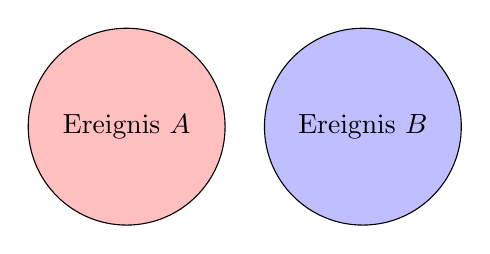
\begin{tikzpicture}
            {
    \def\firstcircle{(0,0) circle (1.25cm)}
    \def\secondcircle{(3,0) circle (1.25cm)}

    \fill[red!25] \firstcircle;
    \fill[blue!25] \secondcircle;

    \draw \firstcircle node {Ereignis $A$};
    \draw \secondcircle node {Ereignis $B$};
}

        \end{tikzpicture}
        \label{fig:disjunkt}
    }
    \subfigure[$A$ und $B$ sind nicht disjunkt]{
        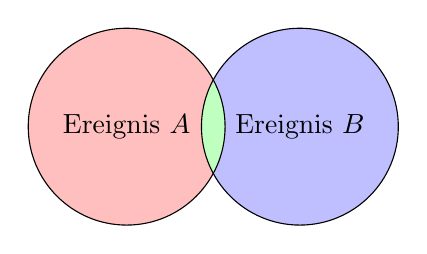
\begin{tikzpicture}
            {
    \def\firstcircle{(0,0) circle (1.25cm)}
    \def\secondcircle{(2.2,0) circle (1.25cm)}

    \fill[red!25] \firstcircle;
    \fill[blue!25] \secondcircle;
    \begin{scope}
        \clip \firstcircle;
        \fill[green!25] \secondcircle;
    \end{scope}

    \draw \firstcircle node {Ereignis $A$};
    \draw \secondcircle node {Ereignis $B$};
}

        \end{tikzpicture}
        \label{fig:nicht_disjunkt}
    }
    \label{fig:teilmengen}
    \caption{Disjunkte und nicht Disjunkte Mengen erklärt}
    \end{figure}

    \begin{satz}[Multiplikationssatz(Multiplikationstheorem)]\index{Multiplikationssatz}:
        \label{satz:multiplikationssatz}
        \index{Multiplikationstheorem|see{Multiplikationssatz}}\\
        Mit dem Multiplikationssatz wird die Wahrscheinlichkeit berechnet, dass
        die Ereignisse  $A_{1},A_{2},...,A_{k}$ gleichzeitig eintreten.

        Dafür drehen wir die Formel der bedingten Wahrscheinlichkeit um und
        erweitern sie:
        \[
            \mathbb{P}\left(A\cap B\right)=\mathbb{P}\left(B\right)\mathbb{P}(A|B)
        \]
    \end{satz}
    Die mehrfache Anwendung dieser Formel liefert:
    \[
        \mathbb{P}\left(A_{1}\cap ... \cap A_{k}\right)=
        \mathbb{P}\left(A_{1}\right)\mathbb{P}\left(A_{2}|A_{1}\right)\mathbb{P}\left(A_{3}|A_{1}\cap A_{2}\right) ... 
        \mathbb{P}\left(A_{k}|A_{1}\cap ... \cap A_{k-1}\right)
    \]

    \textbf{Die Ungleichung von Bonferroni kann das etwa Abschätzen.}\index{Ungleichung!von Bonferroni}\index{Bonferrroni Ungleichung|see{Ungleichung von Bonferroni}}
    \[\mathbb{P}(\bigcap_i A_i)=1-\sum_i\mathbb{P}(A_i^c)\]

    \begin{bsp}[Ziehen ohne Zurücklegen (Multiplikationstheorem)]:\\
    In einer Urne sind zwei schwarze und drei weiße Kugeln. Es wird dreimal
    ohne Zurücklegen gezogen und wir wollen die Wahrscheinlichkeit
    bestimmen, dass alle gezogenen Kugeln weiß sind. 

    Wir setzen also $A_{i}$ gleich dem Ereignis, dass die $i$-te gezogene Kugel weiß ist und suchen
    $\mathbb P(A_{1}\cap A_{2}\cap A_{3})$.

    \begin{tabular}{>{\centering\arraybackslash}p{0.28\linewidth}|>{\centering\arraybackslash}p{0.28\linewidth}|>{\centering\arraybackslash}p{0.28\linewidth}}
        &&\\
        \textbf{Zug 1} & \textbf{Zug 2} & \textbf{Zug 3} \\
            \trimbox{0 0 0 -0.4cm}{
                \begin{tikzpicture}
                    {
\begin{scope}[yshift=-180,yslant=0.5,xslant=-1]
    %circle circumventing the smallest cluster 
    \node[circle,circular glow,fill=red!20,draw=red,thick]
    at (4.4,2.8) {\phantom{perimetro}};
\end{scope}

%atom clusters are rotated for a better visualisation
\begin{scope}[rotate around = {-5:(0,0,0)}]
    \draw[-latex,thick](2,-4)node[below]
        {Ziehe} to[out=90,in=270] (2.3,-2.95);
    \foreach \x  in {6.6,7.1}
        \shadedraw [ball color=black] (\x,2.5,12.8) circle (0.25cm);
    \foreach \x  in {6.5,7,7.5}
        \shadedraw [ball color=white] (\x,2.5,13.5) circle (0.25cm);
\end{scope}
}
%Graphic
                \end{tikzpicture}
            } &
             \trimbox{0 0 0 -0.4cm}{
                \begin{tikzpicture}
                    {
\begin{scope}[yshift=-180,yslant=0.5,xslant=-1]
    %circle circumventing the smallest cluster 
    \node[circle,circular glow,fill=red!20,draw=red,thick]
    at (4.4,2.8) {\phantom{perimetro}};
\end{scope}

%atom clusters are rotated for a better visualisation
\begin{scope}[rotate around = {-5:(0,0,0)}]
    \draw[-latex,thick](2,-4)node[below]
        {Ziehe} to[out=90,in=270] (1.8,-2.95);
    \foreach \x  in {6.6,7.1}
        \shadedraw [ball color=black] (\x,2.5,12.8) circle (0.25cm);
    \foreach \x  in {6.5,7}
        \shadedraw [ball color=white] (\x,2.5,13.5) circle (0.25cm);
\end{scope}
}
%Graphic
                \end{tikzpicture}
            } &
             \trimbox{0 0 0 -0.4cm}{
                \begin{tikzpicture}
                    {
\begin{scope}[yshift=-180,yslant=0.5,xslant=-1]
    %circle circumventing the smallest cluster 
    \node[circle,circular glow,fill=red!20,draw=red,thick]
    at (4.4,2.8) {\phantom{perimetro}};
\end{scope}

%atom clusters are rotated for a better visualisation
\begin{scope}[rotate around = {-5:(0,0,0)}]
    \draw[-latex,thick](2,-4)node[below]
        {Ziehe} to[out=90,in=270] (1.3,-2.95);
    \foreach \x  in {6.6,7.1}
        \shadedraw [ball color=black] (\x,2.5,12.8) circle (0.25cm);
    \foreach \x  in {6.5}
        \shadedraw [ball color=white] (\x,2.5,13.5) circle (0.25cm);
\end{scope}
}
%Graphic
                \end{tikzpicture}
            } \\
            $\mathbb{P}(A_1)=\frac{3}{5}$ & $\mathbb{P}(A_2|A_1)=\frac{2}{4}=\frac{1}{2}$ &$\mathbb{P}(A_3|A_1\cap A_2)=\frac{1}{3}$\\
        &&\\
    \end{tabular}

    Nun wenden wir das Multiplikationstheorem an:
    \[
    \mathbb P\left(A_{1}\cap A_{2}\cap A_{3}\right)=
    \mathbb P\left(A_{1}\right)\mathbb P\left(A_{2}|A_{1}\right)\mathbb P\left(A_{3}|A_{1}\cap A_{2}\right)=
    \frac{3}{5}\cdot \frac{1}{2}\cdot \frac{1}{3}=\frac{1}{10}
    \]

    \end{bsp}

    \index{Bedingte Wahrscheinlichkeit|)}
    
    \section{Stochastische Unabhängigkeit}
    \index{Unabhängigkeit!stochastische|see{stochastische Unabhängigkeit}}
    \index{stochastische Unabhängigkeit|(}

    Zwei Ereignisse heißen stochastisch unabhängig, wenn gilt:

    \[
        \mathbb P\left(A\cap B\right)=
        \mathbb P\left(A\right)\cdot \mathbb P\left(B\right)\text{ bzw. }
        \mathbb P\left(A|B\right)=\mathbb P\left(A\right)=\mathbb P\left(A|B^{C}\right)
    \]
    Die Wahrscheinlichkeit des Eintretens von $A$ hängt nicht davon ab, ob das Ereignis $B$ oder $B^C$ eintritt.

    \begin{bsp} zur Erklärung: \\
        Sie erhalten 10{\texteuro}, falls
        ein geworfenes Kreidestück in der oberen Hälfte der Tafel landet,
        ansonsten verlieren Sie 10{\texteuro}. Dabei stehen Sie in einem
        Nebenraum und überlegen sich, ob Sie die Wette annehmen sollen. In der
        Zwischenzeit wird die Kreide geworfen. Bevor Sie ihre Wette platzieren,
        kommt ein {\quotedblbase}Spion{\textquotedblleft} und erzählt Ihnen,
        dass er für einen gewissen Betrag verrät, ob die Kreide in der linken
        oder rechten Seite der Tafel gelandet ist.\\

        Wie Wertvoll ist diese Information für Sie?\\

        Das Angebot ist für Sie wertlos, denn die Information ändert nichts an Ihrem
        Wissen über den Wettausgang.
    \end{bsp}

    \begin{figure}
    \centering
    \subfigure[$A$ und $B$ sind disjunkt]{
        \begin{tikzpicture}
            {
    \def\firstrect{(-3,-1) rectangle (0,0.5)}
    \def\secondrect{(0,-1) rectangle (3,0.5)}
    \def\rectangle{(-3,-1) rectangle (3,0.5)}

    \fill[red!25] \secondrect;
    \fill[blue!25] \firstrect;

    \draw[black] \firstrect node[below left=0cm and 1.5cm] {\small{Ereig. $A$}};
    \draw[black] \secondrect node[below left] {\small{Ereig. $B$}};
    \draw[black] \rectangle;
}

        \end{tikzpicture}
        \label{fig:tafeln_disjunkt}
    }
    \subfigure[$A$ und $B$ sind nicht disjunkt]{
        \begin{tikzpicture}
            {
    \def\firstrect{(-3,-1) rectangle (1,0.5)}
    \def\secondrect{(-1,-1) rectangle (3,0.5)}
    \def\rectangle{(-3,-1) rectangle (3,0.5)}

    \fill[red!25] \secondrect;
    \fill[blue!25] \firstrect;

    \begin{scope}
        \clip \firstrect;
        \fill[orange] \secondrect;
    \end{scope}

    \draw[black] \firstrect node[below left=0cm and 2.5cm] {\small{Ereig. $A$}};
    \draw[black] \secondrect node[below left] {\small{Ereig. $B$}};
    \node[above] {$A\cap B$};
}

        \end{tikzpicture}
        \label{fig:tafeln_nicht_disjunkt}
    }
    \caption{Disjunkte und nicht disjunkte Tafeln}
    \label{fig:tafeln}
    \end{figure}

    Zur Verdeutlichung siehe Abbildung \ref{fig:tafeln}:
    Die Grundmenge $\Omega$ wird durch den Rahmen dargestellt, darin
    befinden sich die Mengen A und B (disjunkt und überlappend) Es gilt
    $\mathbb P\left(M\right)=1,\mathbb P\left(A\right)=0,5$
    und
    $\mathbb P\left(B\right)=0,5$.

    \begin{multicols}{2}
        Siehe Abbildung \ref{fig:tafeln_disjunkt}\\
        \begin{eqnarray*}
            \mathbb{P}(A\cap B) &=& \mathbb{P}(A)\cdot \mathbb{P}(B)\\
            0 &\neq& 0.25
        \end{eqnarray*}
    Wird $B$ getroffen, ist
    \[\mathbb{P}\left(A|B\right)=0\neq \mathbb P(A)\]
    
    Die Ereignisse sind stochastisch abhängig, dass $B$ getroffen wurde gibt
    uns viel Auskunft über die Wahrscheinlichkeit von $A$.
    
    \columnbreak
        Siehe Abbildung \ref{fig:tafeln_nicht_disjunkt}\\
        \begin{eqnarray*}
            \mathbb{P}(A\cap B) &=& \mathbb{P}(A)\cdot \mathbb{P}(B)\\
            0.25 &=& 0.25
        \end{eqnarray*}

    Wird $B$ getroffen, ist
    \[\mathbb P\left(A|B\right)=0.5=\mathbb P(A)\]

    Die Ereignisse sind stochastisch unabhängig, dass $B$ getroffen wurde,
    gibt uns keine Auskunft über die Wahrscheinlichkeit von $A$.
    \end{multicols}

    \begin{definition}\textbf{Totale Unabhängigkeit}\index{Unabhängigkeit!Totale-|see{Totale Unabhängigkeit}}\index{Totale Unabhängigkeit}\\
        Die $n$ Ereignisse $A_{1},A_{2},...,A_{n}$ heißen total unabhängig, falls für jede Auswahl $A_{1},...,A_{k}$ 
        von $k$ Ereignissen gilt:

        \[
            \mathbb P\left(A_{1}\cap A_{2}\cap ... \cap A_{k}\right)=
            \mathbb P\left(A_{1}\right)\mathbb P\left(A_{2}\right)... \mathbb P(A_{k})
        \]

    \end{definition}

    \begin{definition}\textbf{Paarweise Unabhängigkeit}\index{Unabhängigkeit!Paarweise-|see{Paarweise Unabhängigkeit}}\index{Paarweise Unabhängigkeit}\\
        Die $n$ Ereignisse $A_{1},A_{2},...,A_{n}$ heißen paarweise unabhängig, wenn für alle $1\leq i<j\leq n$ gilt:

        \[
            \mathbb P\left(A_{i}\cap A_{j}\right)=
            \mathbb P\left(A_{i}\right)\mathbb P\left(A_{j}\right)
        \]

    \end{definition}

    \begin{bsp}[aus Wikipedia\cite{wiki:001}]:\\
        In einer Schachtel befinden sich 4 Zettel mit folgenden Zahlenkombinationen: 112, 121, 211, 222. Einer der Zettel wird zufällig (je mit Wahrscheinlichkeit 1/4) gezogen. Wir betrachten dann folgende drei Ereignisse:

            \[A_{1}=\lbrace 1\ {\mathrm {an\ erster\ Stelle}}\rbrace mit \mathbb P(A_{1})={\frac {1}{2}}\]
            \[A_{2}=\lbrace 1\ {\mathrm {an\ zweiter\ Stelle}}\rbrace mit \mathbb P(A_{2})={\frac {1}{2}}\]
            \[A_{3}=\lbrace 1\ {\mathrm {an\ dritter\ Stelle}}\rbrace mit \mathbb P(A_{3})={\frac {1}{2}}\]

        Offensichtlich sind die drei Ereignisse paarweise unabhängig, da gilt

            \[\mathbb P(A_{1}\cap A_{2})=P(A_{1})\cdot \mathbb P(A_{2})={\frac {1}{4}}\]
            \[\mathbb P(A_{1}\cap A_{3})=P(A_{1})\cdot \mathbb P(A_{3})={\frac {1}{4}}\]
            \[\mathbb P(A_{2}\cap A_{3})=P(A_{2})\cdot \mathbb P(A_{3})={\frac {1}{4}}\]

        Die drei Ereignisse sind jedoch nicht (gemeinsam) unabhängig, da gilt

            \[\mathbb P(A_{1}\cap A_{2}\cap A_{3})=0\neq {\frac {1}{8}}=\mathbb P(A_{1})\cdot \mathbb P(A_{2})\cdot \mathbb P(A_{3})\]

        Des Weiteren kann aus $\mathbb P(A_{1}\cap A_{2}\cap A_{3})=\mathbb P(A_{1})\cdot \mathbb P(A_{2})\cdot \mathbb P(A_{3})$ nicht geschlossen werden, dass die drei Ereignisse paarweise unabhängig sind.

    \end{bsp}


    \begin{satz}[von der vollständigen Wahrscheinlichkeit]:\index{Wahrscheinlichkeit!Vollständige-|see{Vollständige Wahrscheinlichkeit}}\index{Vollständige Wahrscheinlichkeit}\index{Totale Wahrscheinlichkeit|see{Vollständige Wahrscheinlichkeit}}\\
    Für den Satz der Vollständigen bzw. totalen Wahrscheinlichkeit brauchen wir folgende Bedingungen:
    \label{satz:vollstaendige_wahrscheinlichkeit}

    \begin{itemize}
        \item Disjunkte Ereignismengen $B_{i}$ von denen $\mathbb P\left(B_{i}\right)$ bekannt ist
        \item $\mathbb P\left(A|B_{i}\right)$ muss bekannt bzw. leicht berechenbar sein
        \item $\sum_{i}{\mathbb P\left(B_{i}\right)}=1$, somit wird die gesamte Grundmenge auf $i$ Flächen aufgeteilt.
    \end{itemize}

    Wir möchten uns also die vollständige Wahrscheinlichkeit berechnen, dass
    $A$ eintrifft. Unser Problem liegt darin, dass wir nur wissen, wie sicher
    $A$ eintrifft, wenn bereits ein anderes Ereignis
    $B_{i}$ eingetroffen ist (bedingte Wahrscheinlichkeit!). Somit ergibt sich:
    \[
        \mathbb P\left(A\right)=\sum _{i}{\mathbb P(B_{i})\mathbb P\left(A|B_{i}\right)}
    \]
    \end{satz}

    \begin{satz}[von Bayes]:\index{Satz von Bayes}\index{Bayes!Satz|see{Satz von Bayes}}\\
        \label{satz:bayes}
        \[\mathbb{P}(A|B)\;\;\Longleftrightarrow\;\;\mathbb{P}(B|A)\]

        Ist die bedingte Wahrscheinlichkeit von $B$ unter $A$, also 
        $\mathbb P\left(B|A\right)$ bekannt, kann mit dem Satz von Bayes
        die Wahrscheinlichkeit von $A$ unter B, also $\mathbb P(A|B)$
        berechnet werden. 
        
        Dafür definieren wir die bedingte Wahrscheinlichkeit
        für beide Fälle, stellen um und erhalten:

        \begin{eqnarray*}
            \mathbb P\left(A|B\right)&=&\frac{\mathbb P\left(B\cap
                A\right)}{\mathbb P\left(B\right)}\Rightarrow \mathbb P\left(B\cap
                A\right)=\mathbb P\left(B\right)\mathbb P(A|B)\\
            \mathbb P\left(B|A\right)&=&\frac{\mathbb P\left(B\cap
                A\right)}{\mathbb P(A)}\Rightarrow \mathbb P\left(B\cap
                A\right)=\mathbb P\left(A\right)\mathbb P(B|A)\\
            \mathbb P\left(B\right)\mathbb P\left(A|B\right)&=&\mathbb P\left(B\cap A\right)=
                \mathbb P\left(A\right)\mathbb P\left(B|A\right)\\
        \end{eqnarray*}
        Somit erhalten wir:
        \[\mathbb P\left(A|B\right)=\frac{\mathbb P\left(B|A\right)\mathbb P\left(A\right)}{\mathbb P(B)}\]
    \end{satz}

    \begin{bsp}\label{bsp:krankheit} \textbf{Krankheit (Vollständige Wahrscheinlichkeit \& Satz von Bayes)}\\

    Von einer Krankheit sind 2\% der Bevölkerung betroffen. Ein Test gibt
    bei einem Kranken mit Wahrscheinlichkeit 0.99 ein positives Ergebnis,
    bei einem Gesunden mit Wahrscheinlichkeit 0.01.

    \begin{enumerate}[a)]
        \item \label{itm:krankheit_a}Bestimmen Sie die Wahrscheinlichkeit, dass eine zufällig gewählte
            Person positiv getestet wird.

            Abbildung \ref{fig:krankheit} beschreibt die Situation Der grüne Rahmen kennzeichnet den
            Wahrscheinlichkeitsbereich für ein positives Testergebnis. Es ist klar
            ersichtlich, dass die Trefferquote bei kranken Personen viel höher ist,
            als bei gesunden. Nun möchten wir die Wahrscheinlichkeit bestimmen,
            dass eine zufällig gewählte Person positiv getestet ist, also im
            grün-strichlierten Bereich liegt.

            \[\mathbb P\left(A\right)=\text{Positiv getestet}\]
            \[\mathbb P\left(B\right)=\text{Negativ getestet}\]
            \[\mathbb P\left(A\right)=\mathbb P\left(B\right)\mathbb P\left(A|B\right)+\mathbb P\left(B^{C}\right)\mathbb P\left(A|B^{C}\right) = 0.98\cdot 0.01+0.02\cdot 0.99=0.0296\approx 3\%\]
            Hier wurde $\mathbb P(A)$ mit dem Satz der Vollständigen Wahrscheinlichkeit berechnet. 
        \item Bestimmen Sie die bedingte Wahrscheinlichkeit dafür, dass eine
            zufällig gewählte Person krank ist, wenn das Testergebnis positiv ist.

            Mit dem Wissen aus \ref{itm:krankheit_a}) kann nun  $P(B^{C}|A)$ berechnet werden.

            \[
                \mathbb P(B^{C}|A)=\frac{\mathbb P(B^{C}\cap A)}{\mathbb P\left(A\right)}=
                \frac{\mathbb P\left(B^{C}\right)\mathbb P(A|B^{C})}{\mathbb P(A)}=\frac{0.02\cdot 0.99}{0.0296}=0.6689\approx 67\%
            \]
            Hier wurde $\mathbb P\left(B^{C}\cap A\right)$ mit dem Satz von Bayes berechnet.
        \end{enumerate}
    \end{bsp}

    \begin{figure}
    \centering
        \begin{tikzpicture}
            {
    \def\firstrect{(-2,-2) rectangle (2,2)}
    \def\secondrect{(0.4,1.6) rectangle (2,2)}
    \def\thirdrect{(0.6,1.4) rectangle (2,2)}

    \fill[red!25] \secondrect;
    \fill[blue!25] \firstrect;

    \begin{scope}
        \clip \firstrect;
        \fill[orange] \secondrect;
    \end{scope}

    \draw[green,dashed,line width=2pt] \thirdrect;
    \draw[black] \firstrect node[below left=1.7 and 0.65] {\small{Gesund (98\%)}};
    \draw[black] \secondrect node[below left=-0.07 and -0.1] {\scriptsize{Krank (2\%)}};
}

        \end{tikzpicture}
        \caption{Krankheit in Bezug auf Testergebnis (grün Strichliert) siehe Beispiel \ref{bsp:krankheit}, (Achtung, übertrieben gezeichnet)}
        \label{fig:krankheit}
    \end{figure}

    \index{stochastische Unabhängigkeit|)}

}
